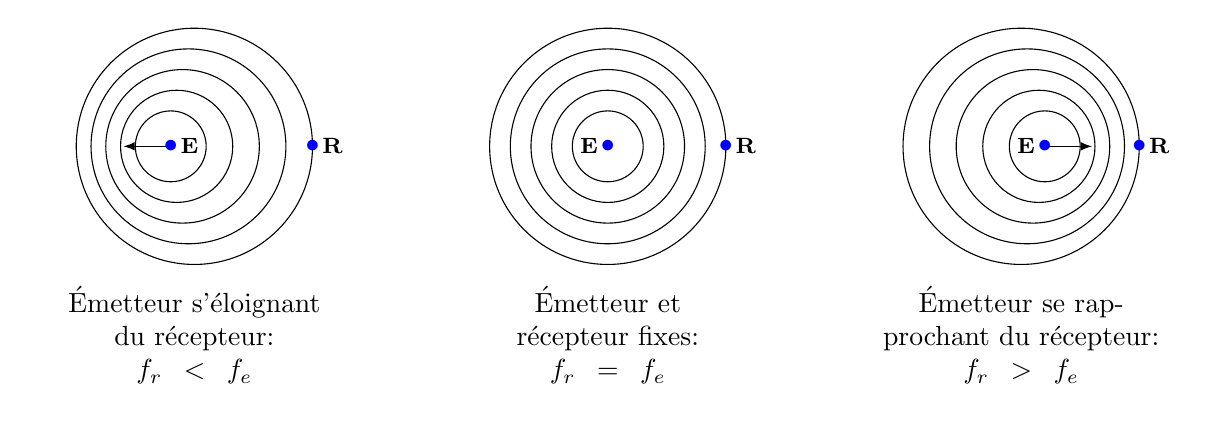
\begin{tikzpicture}[scale=0.75]
  \begin{scope}[shift={(-7,0)}]
    \foreach \i in {0,...,4}{
      \draw (-\i*0.1,0) circle[radius=2-\i*0.35];}

    \draw[-latex] (-.4,0) node[blue]  {$\bullet$} node[right] {\footnotesize{\textbf{E}}} --++(-0.8,0);
    \draw (2,0) node[blue]  {$\bullet$} node[right] {\footnotesize{\textbf{R}}};
    \node[text width=4cm,align=center] at (0,-3.2) {Émetteur s'éloignant du récepteur:\\ $f_r < f_e$};
  \end{scope}

  \begin{scope}
    \foreach \i in {0,...,4}{
      \draw (0,0) circle[radius=2-\i*0.35];}

    \draw (0,0) node[blue]  {$\bullet$} node[left] {\footnotesize{\textbf{E}}};
    \draw (2,0) node[blue]  {$\bullet$} node[right] {\footnotesize{\textbf{R}}};
    \node[text width=4cm,align=center] at (0,-3.2) {Émetteur et récepteur fixes:\\ $f_r = f_e$};
  \end{scope}

  \begin{scope}[shift={(7,0)}]
    \foreach \i in {0,...,4}{
      \draw (\i*0.1,0) circle[radius=2-\i*0.35];}

    \draw[-latex] (0.4,0) node[blue]  {$\bullet$} node[left] {\footnotesize{\textbf{E}}} --++(0.8,0);
    \draw (2,0) node[blue]  {$\bullet$} node[right] {\footnotesize{\textbf{R}}};
    \node[text width=4cm,align=center] at (0,-3.2) {Émetteur se rapprochant du récepteur:\\ $f_r > f_e$};
  \end{scope}
\end{tikzpicture}
